\documentclass[12pt, letterpaper]{../assignment}
\usepackage{graphicx}
\usepackage{courier}
\usepackage{minted}
\usepackage{amsmath}
\usepackage{commath}
\usepackage{amssymb}
\usepackage{amsfonts} 
\usepackage{cancel}
\usepackage{enumitem}
\usepackage{array}

\usepackage{tikz}
\usetikzlibrary{shapes,arrows,positioning}

\usemintedstyle{monokai}
\oddsidemargin = 0pt
\exercisesheet{Module 13}{Practice Assignment}
\student{Austin Barrilleaux}
\courselabel{EN 525.609}
\semester{Fall 2023}
\usepackage[backend=bibtex,style=numeric,sorting=none]{biblatex}
\bibliography{reference}
\usepackage{color}
\definecolor{light-gray}{rgb}{0.2,0.2,0.2}
\setminted{bgcolor=light-gray}
\setlength{\parindent}{0pt}

\makeatletter
\patchcmd{\minted@colorbg}{\noindent}{\medskip\noindent}{}{}
\apptocmd{\endminted@colorbg}{\par\medskip}{}{}
\makeatother

\begin{document}
\subsection*{Problem 1}

\subsubsection*{Solve the following 9th Edition textbook problems:\\
\begin{itemize}
    \item 9-49 (a)
    \item 9-50 (c,d)
\end{itemize}}

\subsubsection*{9-49: Consider that the controller in the liquid-level control system shown in Fig. 9P-10 is a single-stage phase-lag controller:}

$$ \mathbf{ G_c(s) = \frac{1 + a T s}{1 + T s}, \ \ \ a < 1 } $$

$$ \mathbf{ G_p(s) = \frac{10 N}{s(s +1)(s + 10)} } $$

\subsubsection*{(a) For $\mathbf{N = 20}$,
select the values of a and T so that the two complex roots of the characteristic equation correspond to a relative damping ratio of approximately 0.707.
Plot the unit-step response of the output $\mathbf{y(t)}$.
Find the attributes of the unit-step response.
Plot the Bode plot of $\mathbf{G_c(s)G_p(s)}$ and determine the phase margin of the designed system.}

This makes the process:

$$ G_p(s) = \frac{200}{s(s +1)(s + 10)}  $$

The compensated system is:

$$ G_c(s)G_p(s) = \frac{200(1 + a T s)}{s(s +1)(s + 10)(1 + T s)} $$

Rewriting the uncompensated process as:

$$ G_p(s) = \frac{K}{s(s +1)(s + 10)}  $$

$K_\text{SSE}$ to satisfy the SSE requirement is $K_\text{SSE} = 200$.
\\\\
Looking at the root locus of the uncompensated system where $K = 1$,
we can that $K_\text{\%OS}$ for a damping ratio of 0.707 is $K_\text{\%OS} = 4.54$:

\begin{figure}[H]
    \centering
    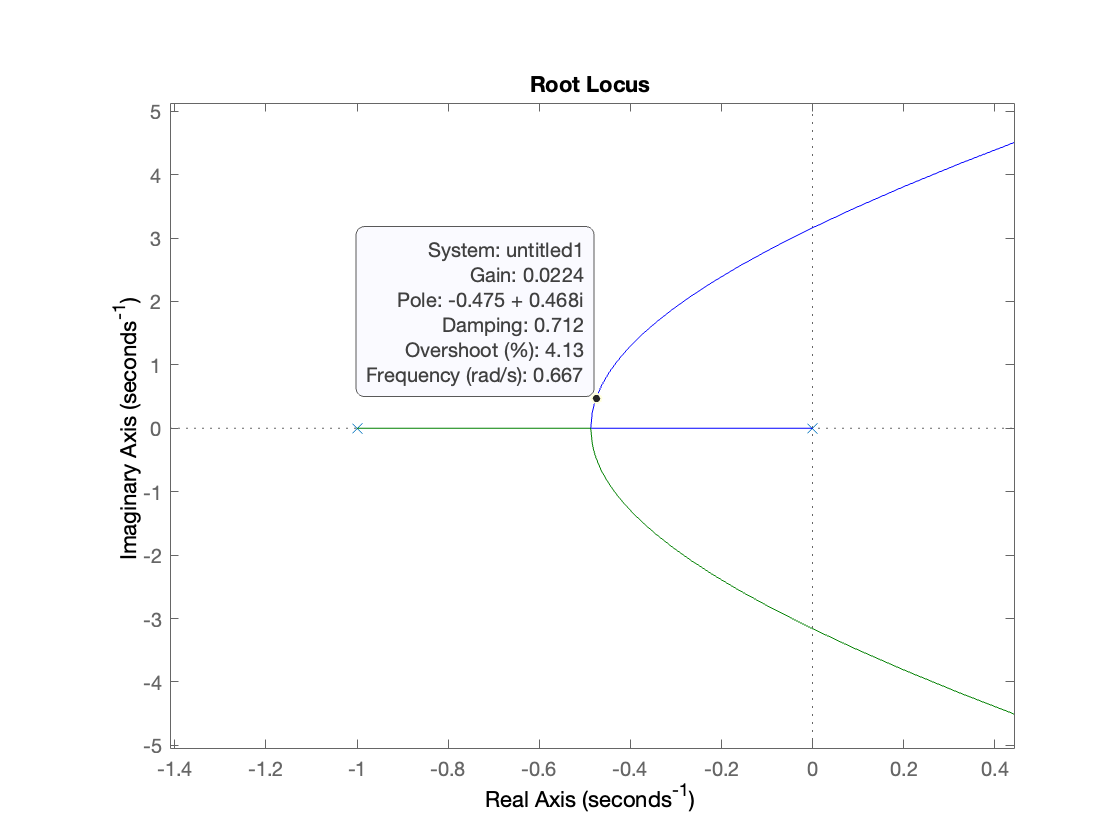
\includegraphics[width=1\linewidth]{./figures/rlocus_9_49a.png}
    \caption{P9-49 (a): Root Locus}
\end{figure}

We can calculate $a$ for the compensated system as:

$$ a = \frac{K_\text{\%OS}}{K_\text{SSE}} = \frac{4.54}{200} = 0.0227 $$

To determine a value for $T$ as a general guideline,
the frequency $\frac{1}{aT}$ should be approximately one decade below $\omega_g'$,
the crossover frequency of the forward path transfer function when $K = K_\text{\%OS}$.
Looking at the bode plot for $ \mathbf{ G_p(s) = \frac{4.54}{s(s +1)(s + 10)} } $ in MATLAB:

\begin{figure}[H]
    \centering
    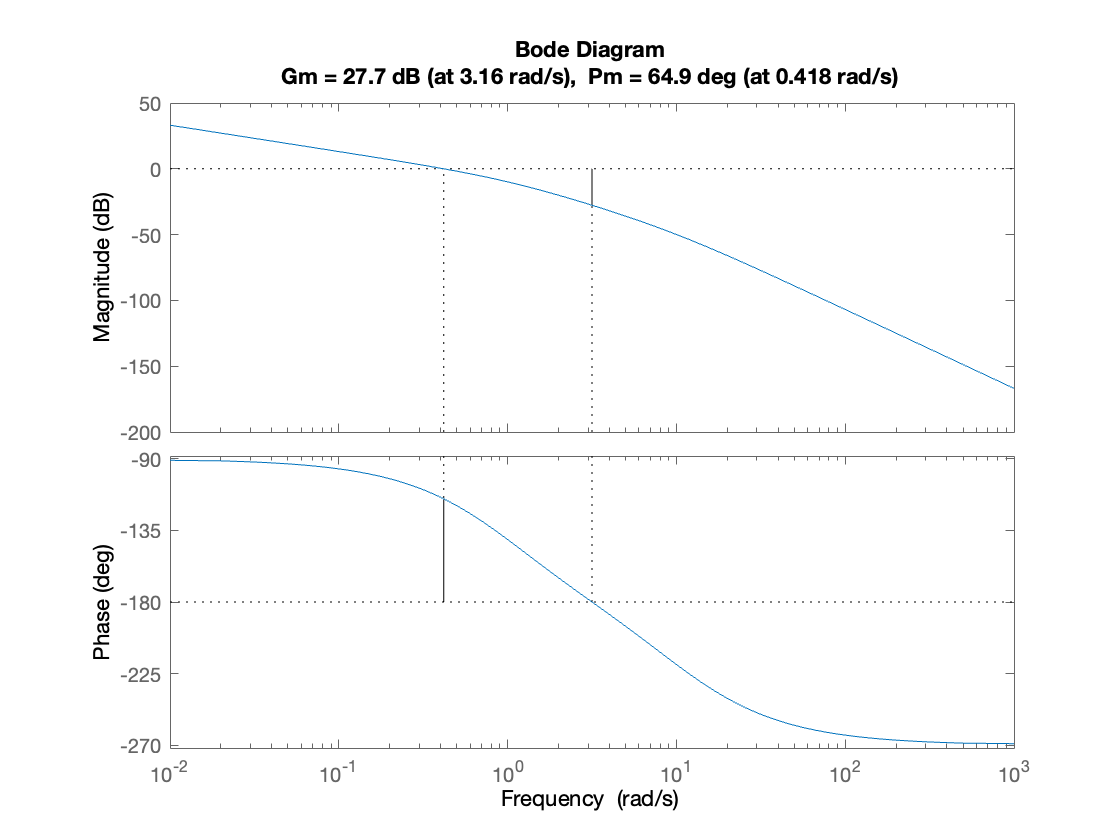
\includegraphics[width=1\linewidth]{./figures/bode_prime_9_49a.png}
    \caption{P9-49 (a): Bode Plot, $G_p$, $K = 4.54$}
\end{figure}

Therefore, $T$ should be calculated as:

$$ T = \left(\frac{\omega_g' a}{10}\right)^{-1}
     = \left(\frac{(0.418)(0.0227)}{10}\right)^{-1}
     = 1053.90 \approx 1050$$

\begin{answer}
    $$ a = 0.0227  \ \text{and} \ T = 1050 $$
\end{answer}

Looking at the closed-loop step-response of the system in MATLAB:

\begin{figure}[H]
    \centering
    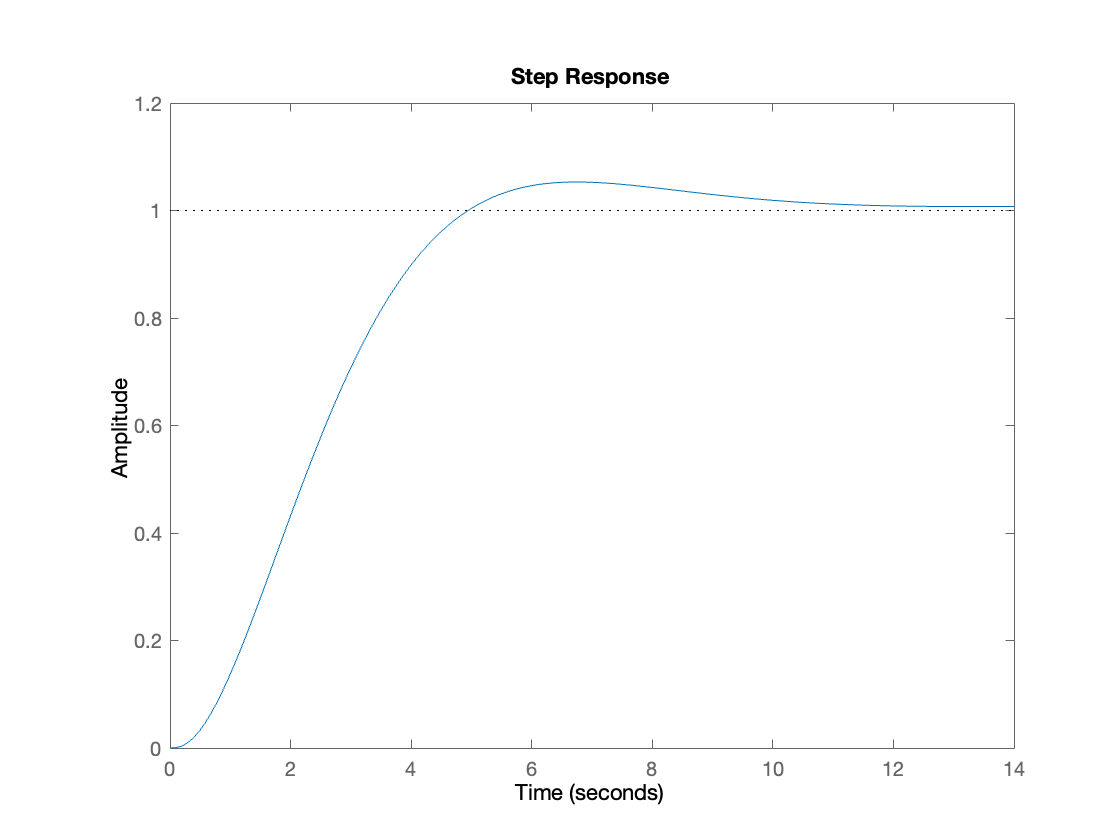
\includegraphics[width=1\linewidth]{./figures/step_9_49a.png}
    \caption{P9-49 (a): Step Response}
\end{figure}

The attributes of the unit-step response,
using the \texttt{stepinfo()} function in MATLAB, are:

\begin{answer}
$$ \texttt{stepinfo()} =  \left[
\begin{array}{rl}
    \textbf{RiseTime:}& 2.8926\\
    \textbf{TransientTime:}& 38.05733\\
    \textbf{SettlingTime:}& 38.05733\\
    \textbf{SettlingMin:}& 0.9061\\
    \textbf{SettlingMax:}& 1.1325\\
    \textbf{Overshoot:}& 13.2498\\
    \textbf{Undershoot:}& 0\\
    \textbf{Peak:}& 1.1325\\
    \textbf{PeakTime:}& 6.8196
\end{array} \right] $$
\end{answer}

Plotting the Bode plot for the forward path transfer function, $G_c(s) G_p(s)$, where:

$$ G_c(s)G_p(s) = \frac{4.54(s + 0.041)}{s (s +1)(s + 10)(s + 0.00095)} $$

We get the plot:

\begin{figure}[H]
    \centering
    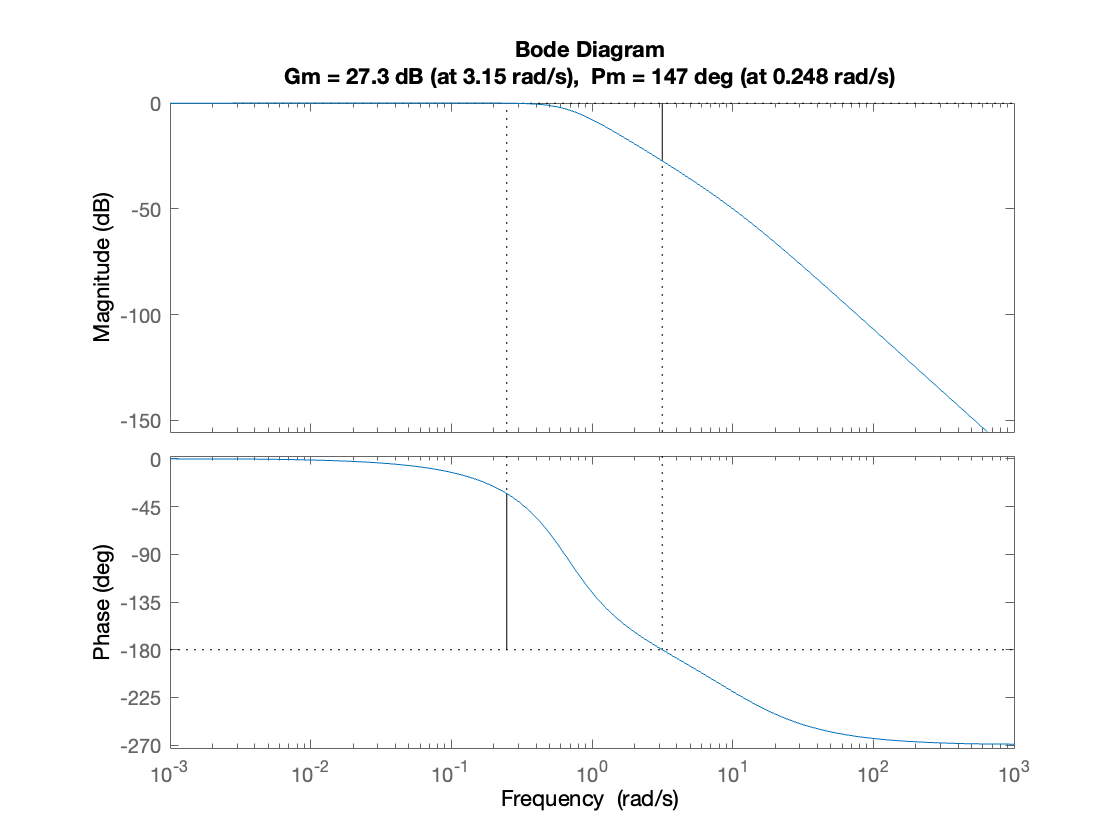
\includegraphics[width=1\linewidth]{./figures/bode_9_49a.png}
    \caption{P9-49 (a): Bode Plot}
\end{figure}

\begin{answer}
The Gain and Phase Margin of the system, respectively, are $GM = 27.3 \ \textbf{dB}$ and $PM = 59.2^\circ$.
\end{answer}

\subsubsection*{9-50: The controlled process of a unity-feedback control system is:
$$ \mathbf{ G_p(s) = \frac{K}{s (s+5)^2 }  } $$
The series controller has the transfer function:
$$ \mathbf{ G_c(s) = \frac{1 + a T s}{1 + T s}  } $$}

\subsubsection*{(c) Design a phase-lag controller ($\mathbf{a< 1}$) so that the following performance specifications are satisfied:\\
\begin{itemize}
    \item Ramp-error constant $\mathbf{K_v= 10}$
    \item Maximum Overshoot $\mathbf{< 1}$ \%
    \item Rise time, $\mathbf{t_r < 2}$ sec
    \item Settling time, $\mathbf{ts < 2.5}$ sec
\end{itemize}
Find the $PM$, $GM$, $M_r$ and $BW$ of the designed system.}


For the system, since $ K_v = 10 $, we can solve for $K$ via the following:

$$ K_v = \lim_{s \to 0} s G(s)
       = \frac{K(1 + a T s)s}{s (s+5)^2 (1 + T s)}
       = \frac{K}{5^2} = 10 $$

Solving for $K$, $K = 250$, which is $K_\text{SSE}$ to satisfy the SSE requirement.
\\
To calculate the damping ratio, $\zeta$ that would yield a 1\% overshoot, we can use the formula:

$$ \zeta = \frac{-\log \left(\frac{\text{\%OS}}{100}\right)}{\sqrt{\pi^2 + \log \left(\frac{\text{\%OS}}{100}\right)^2}}
         = \frac{-\log \left(\frac{1}{100}\right)}{\sqrt{\pi^2 + \log \left(\frac{1}{100}\right)^2}}
         = 0.826 $$ 

Looking at the root locus of the uncompensated system where $K = 1$,
we can that $K_\text{\%OS}$ for a damping ratio of 0.826 is $K_\text{\%OS} = 24.5$:

\begin{figure}[H]
    \centering
    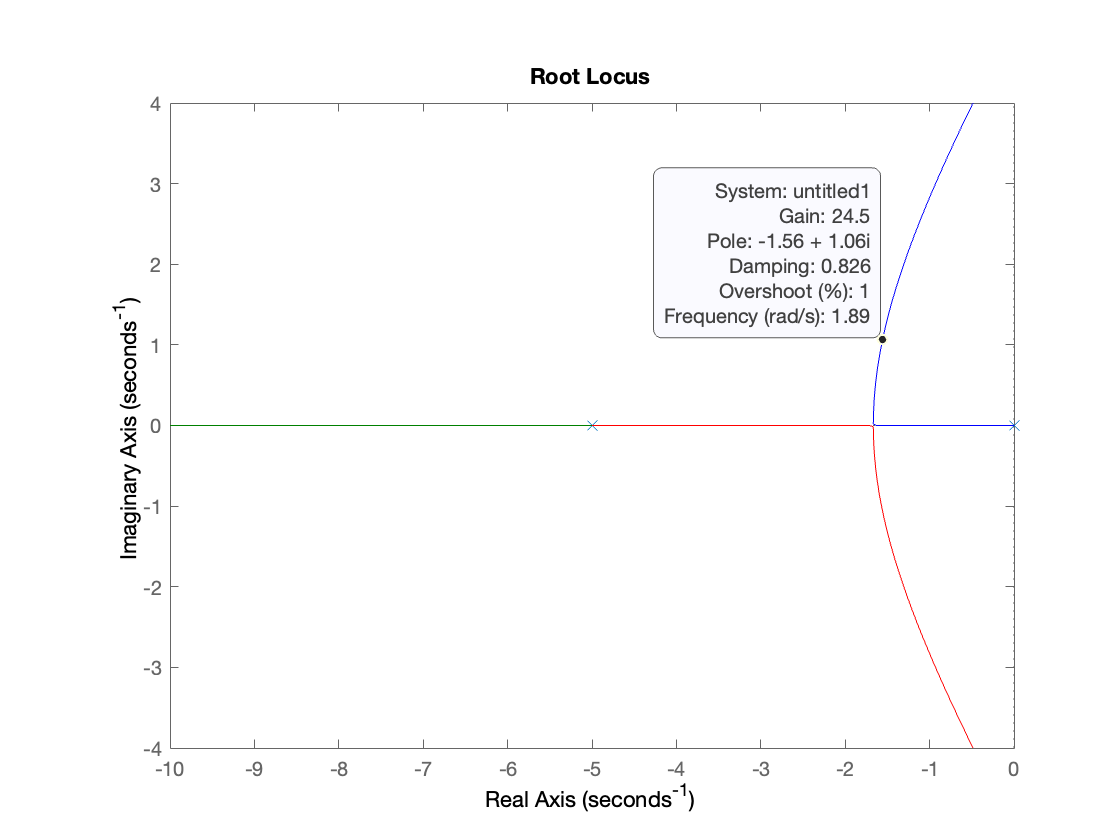
\includegraphics[width=1\linewidth]{./figures/rlocus_9_50c.png}
    \caption{P9-50 (c): Root Locus}
\end{figure}

We can calculate $a$ for the compensated system as:

$$ a = \frac{K_\text{\%OS}}{K_\text{SSE}} = \frac{24.5}{250} = 0.098 $$

To get a $K$ that will satisfy both \%OS and $t_r$, we will apply a fudge factor,
$\gamma$ of 2\% to this value:

$$ a = \gamma \frac{K_\text{\%OS}}{K_\text{SSE}}
= \left(\frac{1}{1+\text{SM}}\right) \frac{K_\text{\%OS}}{K_\text{SSE}}
= \left(\frac{1}{1.02}\right) \frac{24.5}{250} = 0.0961 $$

As in the above problem, to determine a value for $T$ as a general guideline,
the frequency $\frac{1}{aT}$ should be approximately one decade below $\omega_g'$,
the crossover frequency of the forward path transfer function when $K = K_\text{\%OS}$.
Looking at the bode plot for $ \mathbf{ G_p(s) = \frac{250a}{s (s+5)^2 } } $ in MATLAB:

\begin{figure}[H]
    \centering
    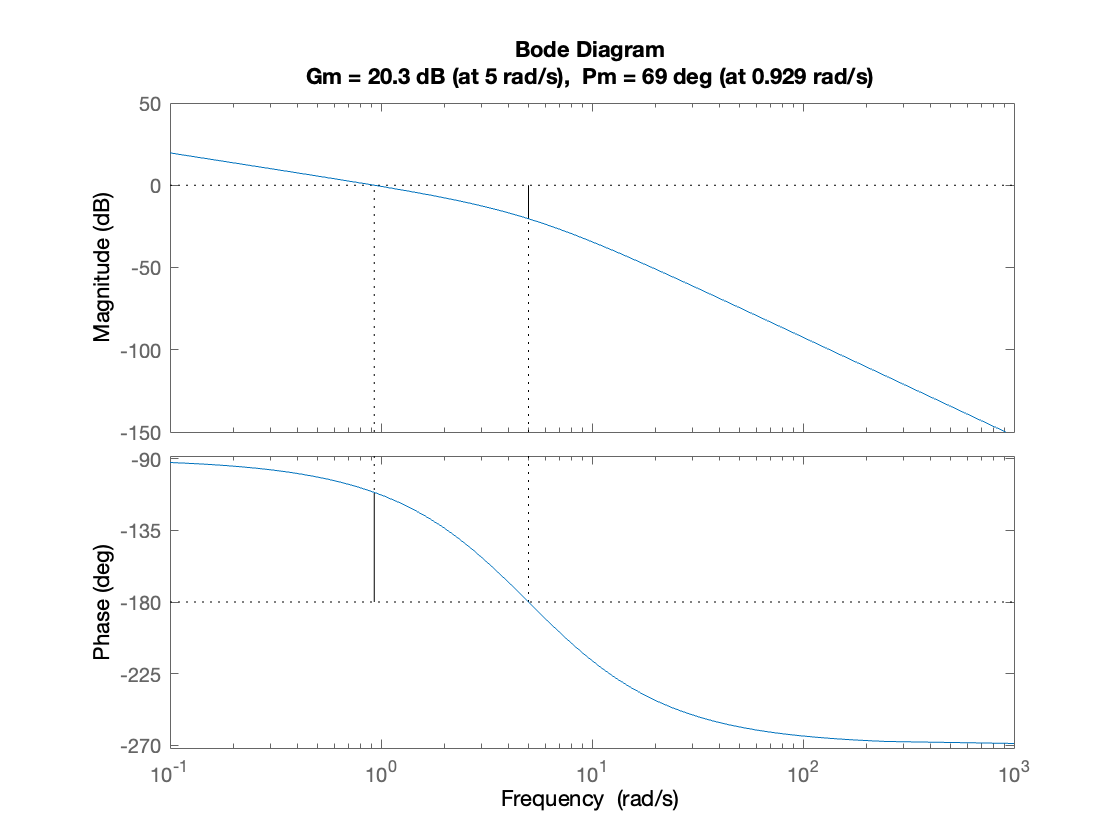
\includegraphics[width=1\linewidth]{./figures/bode_prime_9_50c.png}
    \caption{P9-50 (c): Bode Plot, $G_p$, $K = 250(0.0961)$}
\end{figure}

Therefore, $T$ should be initially calculated as:

$$ T = \left(\frac{\omega_g' a}{10}\right)^{-1}
     = \left(\frac{(0.929)(0.0961)}{10}\right)^{-1}
     = 112.03 \approx 100$$

The attributes of the unit-step response at this value of $T$,
using the \texttt{stepinfo()} function in MATLAB, are:

% \begin{answer}
$$ \texttt{stepinfo()} =  \left[
\begin{array}{rl}
    \textbf{RiseTime:}& 1.2694\\
    \textbf{TransientTime:}&  16.3925\\
    \textbf{SettlingTime:}&  16.3925\\
    \textbf{SettlingMin:}&  0.9026\\
    \textbf{SettlingMax:}&  1.0962\\
    \textbf{Overshoot:}&  9.6168\\
    \textbf{Undershoot:}&  0\\
    \textbf{Peak:}&  1.0962\\
    \textbf{PeakTime:}&  3.2774
\end{array} \right] $$

This value of $T$ does not provide an ideal response for the system,
as overshoot and settling time are too high. From here,
if we continuously increase $T$ by 100 until we get an acceptable response,
we see that when $T = 4400$, all of the requirements are pulled into range.
To provide a little extra cushion, when $T = 4500$:

$$ \texttt{stepinfo()} =  \left[
\begin{array}{rl}
    \textbf{RiseTime:}& 1.4394\\
    \textbf{TransientTime:}& 2.3314\\
    \textbf{SettlingTime:}& 2.3314\\
    \textbf{SettlingMin:}& 0.9051\\
    \textbf{SettlingMax:}& 1.0099\\
    \textbf{Overshoot:}& 0.9908\\
    \textbf{Undershoot:}& 0\\
    \textbf{Peak:}& 1.0099\\
    \textbf{PeakTime:}& 3.2681
\end{array} \right] $$

The values of $a$ and $T$ for a response that meets the requested requirements:

\begin{answer}
    $$ a = 0.0961  \ \text{and} \ T = 4500 $$
\end{answer}


For this design of the unity feedback system:
$$ G_c(s)G_p(s) = \frac{24.01(s + 0.0023)}{s (s +5)^2(s + 0.0002)} $$

The closed-loop step-response can be seen in the following MATLAB plot:

\begin{figure}[H]
    \centering
    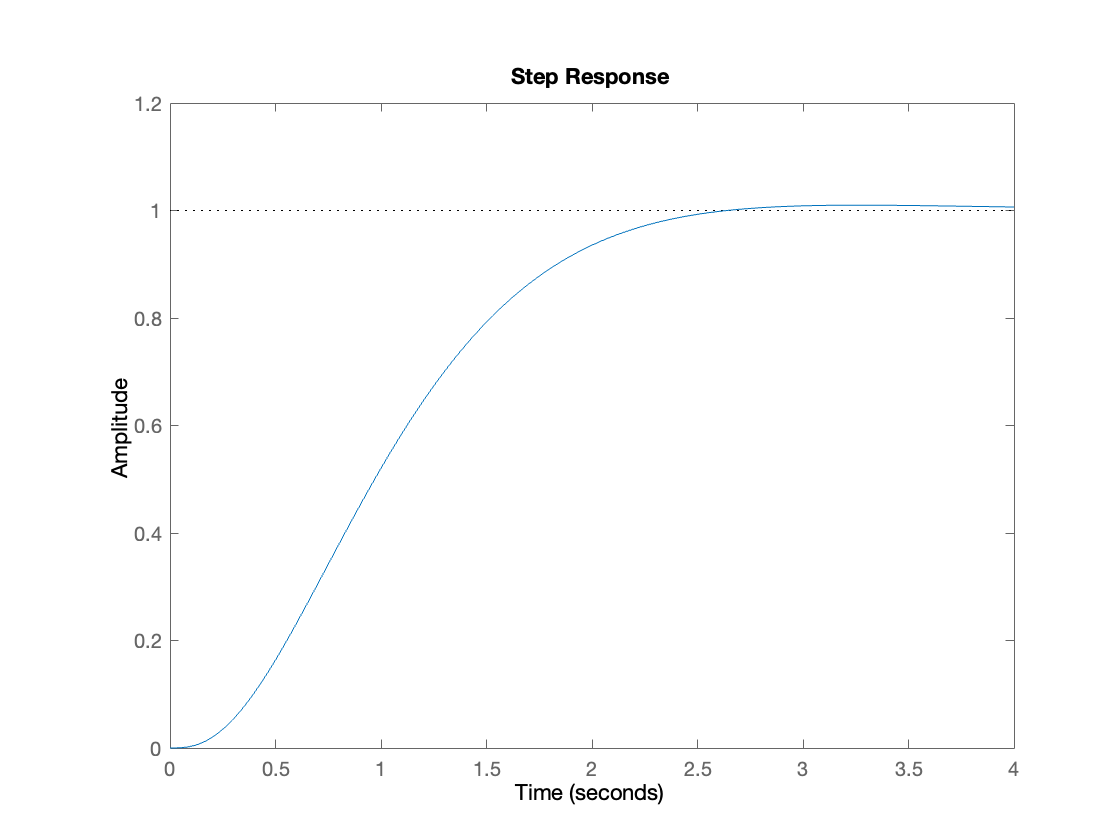
\includegraphics[width=1\linewidth]{./figures/step_9_50c.png}
    \caption{P9-50 (c): Step Response}
\end{figure}

Gain and Phase Margin for the system can be found using the $\texttt{margin()}$ function in MATLAB:

\begin{answer}
$$ \texttt{[GM, PM] = margin():} \left[
\begin{array}{rl}
    GM = & 20.3402 \ \textbf{dB}\\
    PM = & 68.8257^\circ
\end{array} \right] $$
\end{answer}

$M_r$ for the system can be found using the $\texttt{getPeakGain()}$ function in MATLAB:

\begin{answer}
    $$ \texttt{MR = getPeakGain():} \left[M_r = 1.0011\right] $$ 
\end{answer}

$BW$ for the system can be found using the $\texttt{bandwidth()}$ function in MATLAB:

\begin{answer}
    $$ \texttt{BW = bandwidth():} \left[BW = 1.4883 \ \textbf{rad/sec}\right] $$ 
\end{answer}

\subsubsection*{(d) Design the phase-lag controller in the frequency domain so that the following performance specifications are satisfied:
\begin{itemize}
    \item Ramp-error constant $\mathbf{K_v= 10}$
    \item Phase margin $\mathbf{\ge 70^\circ}$
\end{itemize}
Check the unit-step response attributes of the designed system and compare with those obtained in part (c).}

Note that, as in part (c), $K = 250$.
\\\\
The Bode plot of the uncompensated system, $ G(s) = \frac{250}{s (s+5)^2 } $ is:

\begin{figure}[H]
    \centering
    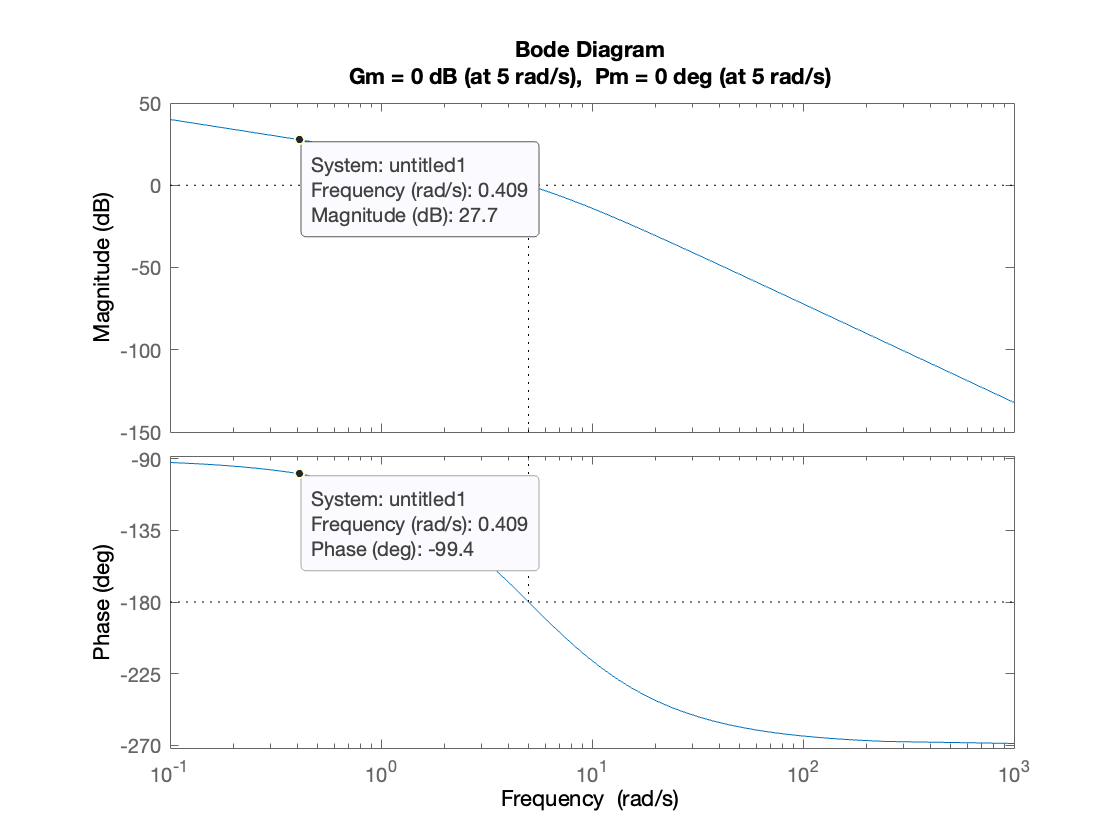
\includegraphics[width=1\linewidth]{./figures/bode_prime_9_50d.png}
    \caption{P9-50 (d): Bode Plot, $G_p$, $K = 250$}
\end{figure}

If we want to make the Phase Margin of the system $\ge 70^\circ$,
since phase margin is initially zero, we need to increase the phase margin by more than $70^\circ$.
To add margin, we will increase it by $~80^\circ$.
To do so, looking at the Bode plot, we see that to get a phase margin of $~80^\circ$,
we must increase the gain margin by 27.7 dB.
\\\\
This allows us to solve for the controller value of $a$ as:

$$ a = 10^{\left( \frac{-GM}{20} \right)} = 10^{\left( \frac{-27.7}{20} \right)} = 0.0412 $$

If we set the value for $\frac{1}{aT}$ to be approximately one decade below $\omega_g'$,
the crossover frequency of the forward path transfer function,
$T$ is calculated as:

$$ T = \left(\frac{\omega_g' a}{10}\right)^{-1}
     = \left(\frac{(0.409)(0.0412)}{10}\right)^{-1}
     = 593.4436 \approx 600$$

\begin{answer}
    $$ a = 0.0412  \ \text{and} \ T = 600 $$
\end{answer}

For this design of the unity feedback system:

$$ G_c(s)G_p(s) = \frac{9.89(s + 0.0404)}{s (s +5)^2(s + 0.0017)} $$


The attributes of the unit-step response  for these values of $a$ and $T$,
using the \texttt{stepinfo()} function in MATLAB, are:

% \begin{answer}
$$ \texttt{stepinfo()} =  \left[
\begin{array}{rl}
    \textbf{RiseTime:}& 3.6073\\
    \textbf{TransientTime:}&  41.6464\\
    \textbf{SettlingTime:}&  41.6464\\
    \textbf{SettlingMin:}&  0.9001\\
    \textbf{SettlingMax:}&  1.0705\\
    \textbf{Overshoot:}&  7.0494\\
    \textbf{Undershoot:}&  0\\
    \textbf{Peak:}&  1.0705\\
    \textbf{PeakTime:}&  11.4026
\end{array} \right] $$

In part (c), the rise and settling times for the response were much faster,
and the overshoot for this response was significantly higher at about 7\%.
Given that the system in part (c) nearly met the $70^\circ$ PM requirement,
it's design has a much more desirable response.
\\\\
A plot of the step-response of the closed-loop system can be seen in the following MATLAB plot:

\begin{figure}[H]
    \centering
    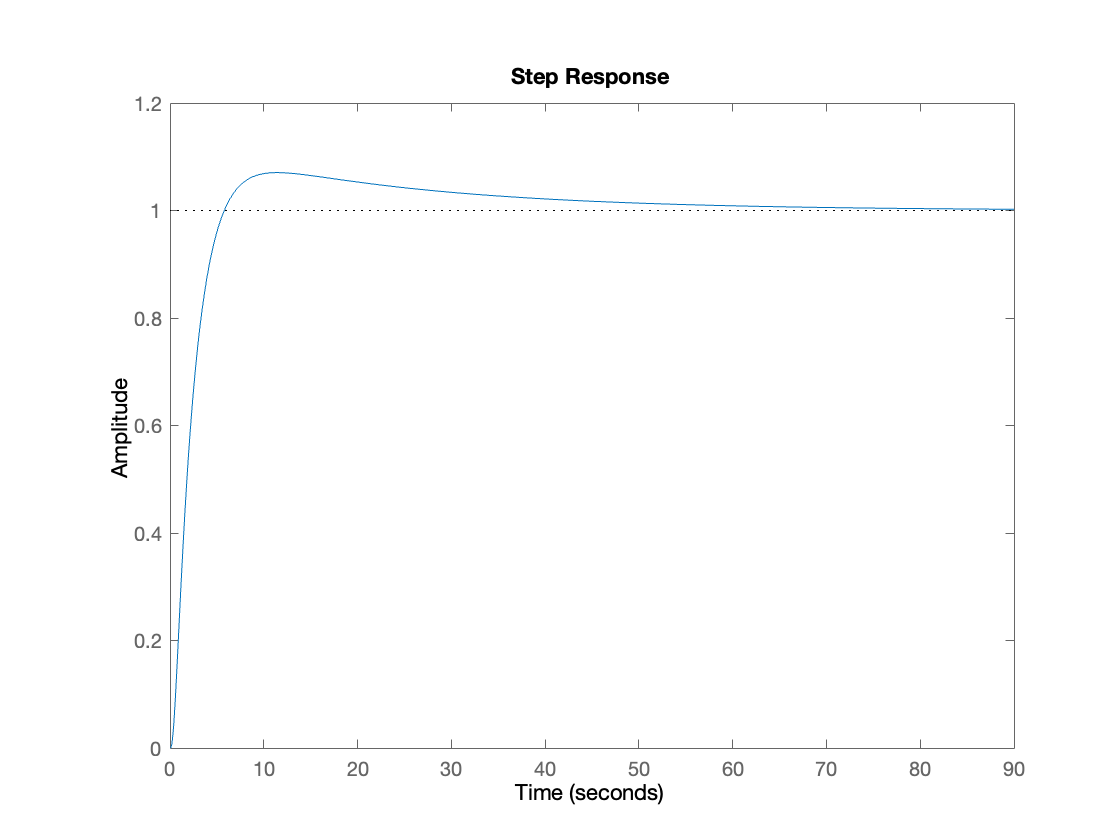
\includegraphics[width=1\linewidth]{./figures/step_9_50d.png}
    \caption{P9-50 (d): Step Response}
\end{figure}



% \end{answer}

% Which can also be written as:

% $$ G_c(s)G_p(s) = \frac{200a(s+\frac{1}{a T})}{s(s +1)(s + 10)(s+\frac{1}{T})} $$

% Looking at a zoomed in view of the root locus plot for the uncompensated system made using the \texttt{rlocus()} function in MATLAB,
% we can see what the complex conjugate roots look like when the damping ratio is roughly equal to $\cos(45^\circ) \approx 0707$:

% \begin{figure}[H]
%     \centering
%     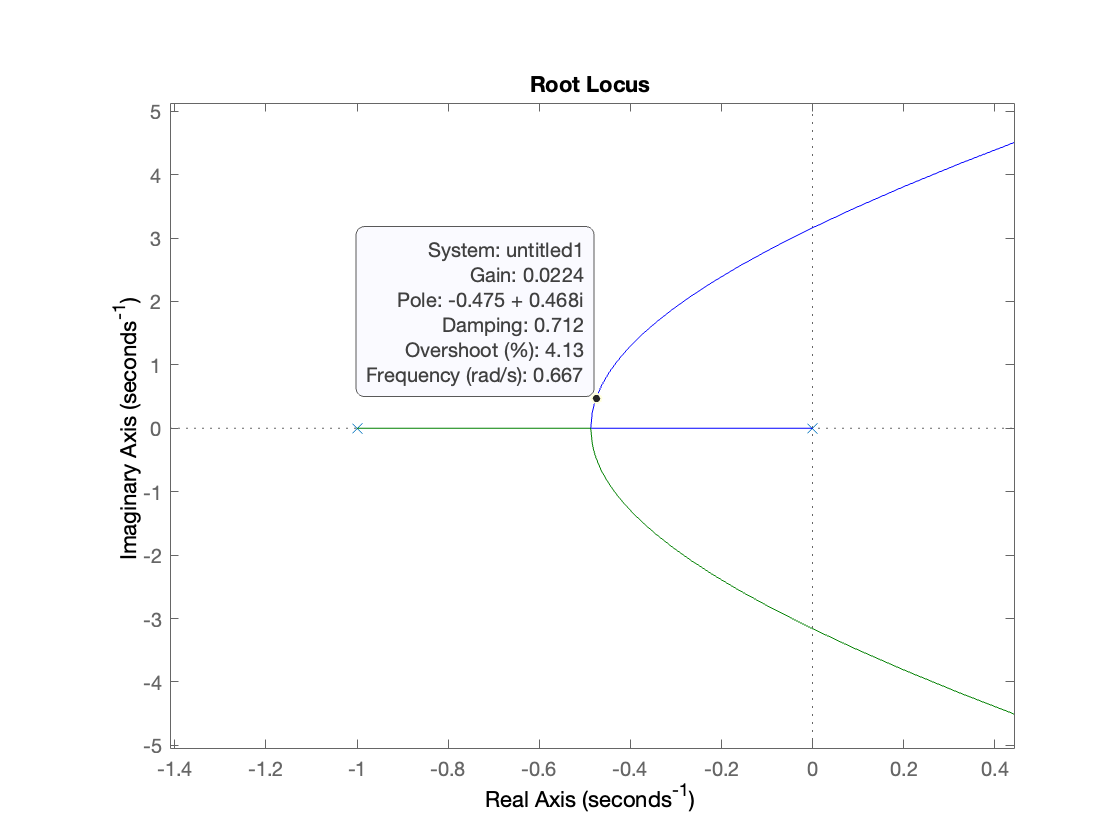
\includegraphics[width=0.7\linewidth]{./figures/rlocus_9_49a.png}
%     \caption{Root Locus}
% \end{figure}

% If we make the assumption that $ \frac{1}{a T} = \frac{1}{T} $, we can write $G(s)$ as:

% $$ G_c(s)G_p(s) = \frac{200a}{s(s +1)(s + 10)} $$

% Using this equation we can solve for $a$ using the following MATLAB code:

% \color{white}
% \hspace*{6em}\inputminted[frame=leftline,fontsize=\footnotesize,
% firstline=8,lastline=29]{matlab}
% {./matlab/P9_49.m}
% \color{black}

% Not that the above algorithm only works given good initial boundaries.

% This solves for a value for $a$ of $a = 0.02268$, where $\zeta - \cos(45^\circ) = -2.22 \cdot 10^{-16}.
% $

% \color{white}
% \hspace*{6em}\inputminted[frame=leftline,fontsize=\footnotesize]{matlab}
% {./matlab/Problem_5_18.m}
% \color{black}

% \begin{figure}[H]
%     \centering
%     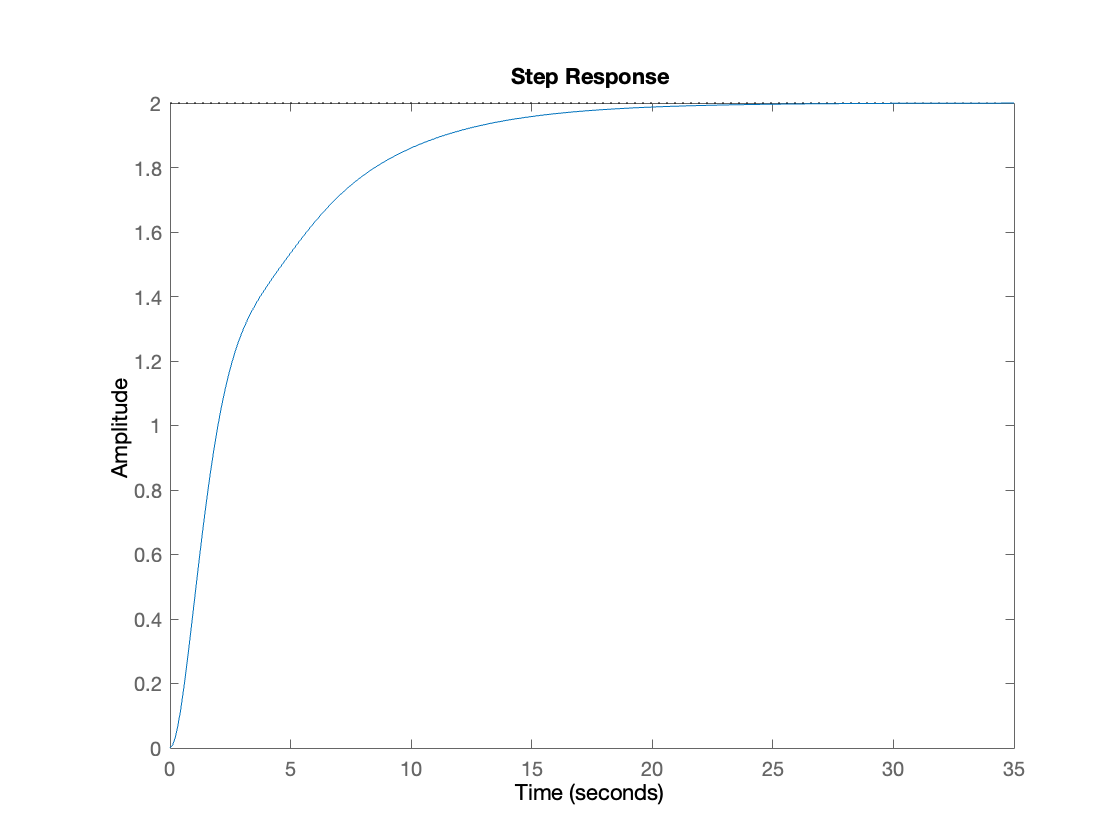
\includegraphics[width=0.7\linewidth]{./figures/step_response.png}
%     \caption{Step Response}
%     \label{fig:step}
%  \end{figure}



\end{document}

